\begin{figure}
\vspace{-4pt}
    \begingroup
    \setlength{\tabcolsep}{1pt}
    \centering
    \begin{tabular}{@{\hskip 0pt}cc@{\hskip 0pt}cc@{\hskip 0pt}}
         \rotatebox[origin=c]{90}{\fontsize{6}{5}\selectfont{Validation Acc. \%}} &  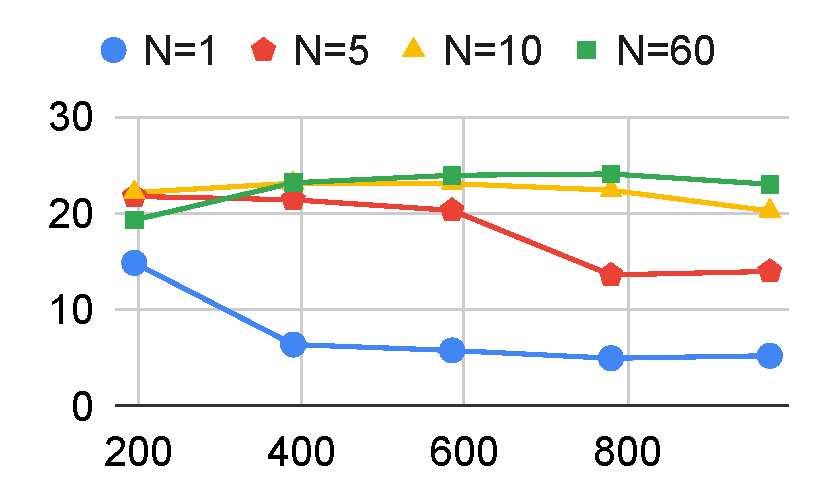
\includegraphics[align=c,width=0.455\linewidth,trim=20 0 0 0,clip]{figures/MandN.pdf}& \hfill\;\;\rotatebox[origin=c]{90}{\fontsize{6}{5}\selectfont{Param. Distance to Target}} &  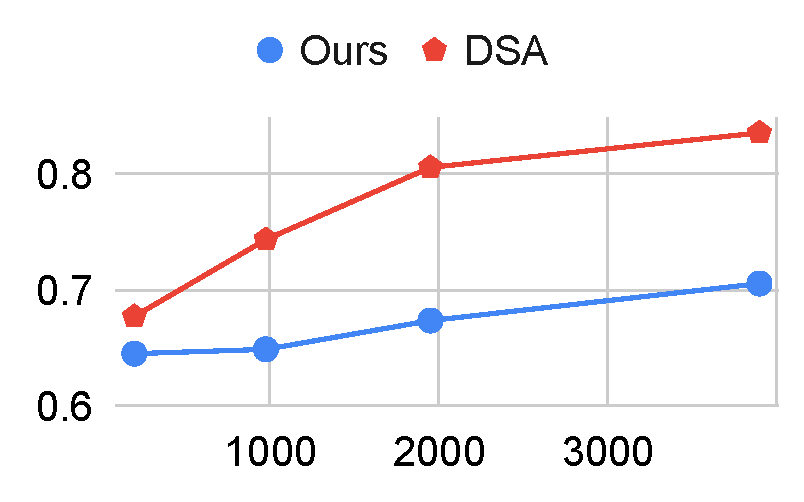
\includegraphics[align=c,width=0.458\linewidth,trim=13 0 9 0,clip]{figures/min_dt.pdf}\\[-1.3ex]
         & \fontsize{6}{5}\selectfont{\;\;\;\;\;$M$: Expert Steps} & & \fontsize{6}{5}\selectfont{\;\;$\Delta t$: Expert Steps between Init.~and Target}
    \end{tabular}
    \endgroup
        \vspace{-9pt}
    \caption{CIFAR-100 (1 image / class). \textbf{Left:} Smaller $M$ and $N$ match shorter-range behavior, which performs worse than longer-range matching. 
    \textbf{Right:} Over $1000$ training steps on distilled data, we track the closest distance in parameter space (normalized MSE in \refeq{weight_matching}) to a target set of parameters, obtained with $\Delta_t$ training steps on real data. Matching long-range behavior, our method better approximate real data training for longer ranges (large $\Delta_t$).
    }
    \lblfig{mn-alpha}
    \vspace{-5pt}
\end{figure}